
\documentclass[11pt,a4paper]{article}


\usepackage[portuguese]{babel}
\usepackage[version=3]{mhchem} % Package for chemical equation typesetting
\usepackage{siunitx} % Provides the \SI{}{} and \si{} command for typesetting SI units
\sisetup{
	load-configurations=binary,
	detect-all,
	group-digits=false,
	output-decimal-marker={,},
	per-mode=symbol,
	per-symbol=/,
	binary-units = true
}
\usepackage{graphicx} % Required for the inclusion of images
\usepackage{natbib} % Required to change bibliography style to APA
\usepackage{amsmath} % Required for some math elements 

\usepackage{multirow}
\usepackage{longtable}
\usepackage{tabto}
\usepackage{booktabs}
\usepackage[utf8]{inputenc}
%\setlength\parindent{0pt} % Removes all indentation from paragraphs

\renewcommand{\labelenumi}{\alph{enumi}.} % Make numbering in the enumerate environment by letter rather than number (e.g. section 6)
\usepackage{epstopdf}
\graphicspath{{figures/}}

\usepackage[colorlinks = true,
linkcolor = blue,
urlcolor  = blue,
citecolor = blue,
anchorcolor = blue]{hyperref}

\usepackage[capitalise]{cleveref}



%\usepackage{times} % Uncomment to use the Times New Roman font

%----------------------------------------------------------------------------------------
%	DOCUMENT INFORMATION
%----------------------------------------------------------------------------------------

\title{Transmissão de imagem entre dispositivos HDMI} % Title
%\version{Edição 1.0}
%\title{Edição 1.0}
\author{INESC-TEC}

\date{\today \\ v1.0} % Date for the report

\begin{document}
	
	\maketitle % Insert the title, author and date
	
	% Please add the following required packages to your document preamble:
	% \usepackage{booktabs}
	\begin{table}[h!]
		\centering
		\label{my-label}
		\begin{tabular}{@{}llll@{}}
			\toprule
			\multicolumn{1}{c}{\textbf{Data}} & \multicolumn{1}{c}{\textbf{Autor}} & \multicolumn{1}{c}{\textbf{Edição}} & \multicolumn{1}{c}{\textbf{Alterações}} \\ \midrule
			11 julho 2017                     & Marisa Oliveira                    & 1.0                                 & Lançamento Inicial                       \\ \bottomrule
		\end{tabular}
	\end{table}
	
	% If you wish to include an abstract, uncomment the lines below
	%\begin{abstract}
	%% Abstract text
	%\end{abstract}
	
	%----------------------------------------------------------------------------------------
	%	SECTIONs
	%----------------------------------------------------------------------------------------
	
	\section{Introdução}
	
	Este manual apresenta os aspetos relevantes sobre a arquitetura implementada em FPGA que permite a transmissão de imagem entre dispositivos HDMI.
	
	\section{Objetivo}
	
	Esta arquitetura tem como principal objetivo a transmissão direta entre a FPGA e o dispositivo final HDMI, tal como mencionado em \cite{R041}. É gerada uma barra de cores em \textit{FULL HD} com uma taxa de atualização vertical de \SI{60}{\hertz} no módulo ``\textit{colorBar\_generator.v}'' e os dados referentes à imagem são transmitidos para a placa HDMI TX, tal como se visualiza na \cref{fig:planoA}.

	\section{Material Utilizado}
	Para a implementação desta arquitetura são utilizados vários equipamentos, entre os quais os seguintes:
	\subsection{FPGA VC7203}
	É uma FPGA (\textit{Field-programmable gate array}) que se caracteriza pelo seu elevado número de recursos e também pelas entradas em saídas de alta velocidade que possui, tal como indica \cite{R008}. É utilizada para implementação do código desenvolvido em Verilog para esta arquitetura e ainda para conexão à placa HDMI pelos conectores FMC (\textit{FPGA Mezzanine Card}).
	\subsection{TB-FMCH-HDMI2-TX}
	Esta placa HDMI caracteriza-se pela capacidade de transmissão de dados HDMI através da receção dos dados referentes à imagem em paralelo. Esses dados são recebidos através dos conectores FMC de interface entre a placa e a FPGA VC7203. Para esta implementação, a placa deve estar configurada por omissão cujos detalhes se encontram em \cite{R009}.
	
	\section{Arquitetura}
	
	O diagrama de blocos na \cref{fig:planoA} representa a arquitetura desenvolvida. É implementado um módulo que gera uma barra de cores em FULL HD com uma taxa de atualização vertical de 60 Hz. Os dados são transmitidos para a placa HDMI transmissora através dos conectores FMC.
	\begin{figure}[h!]
		\begin{center}
			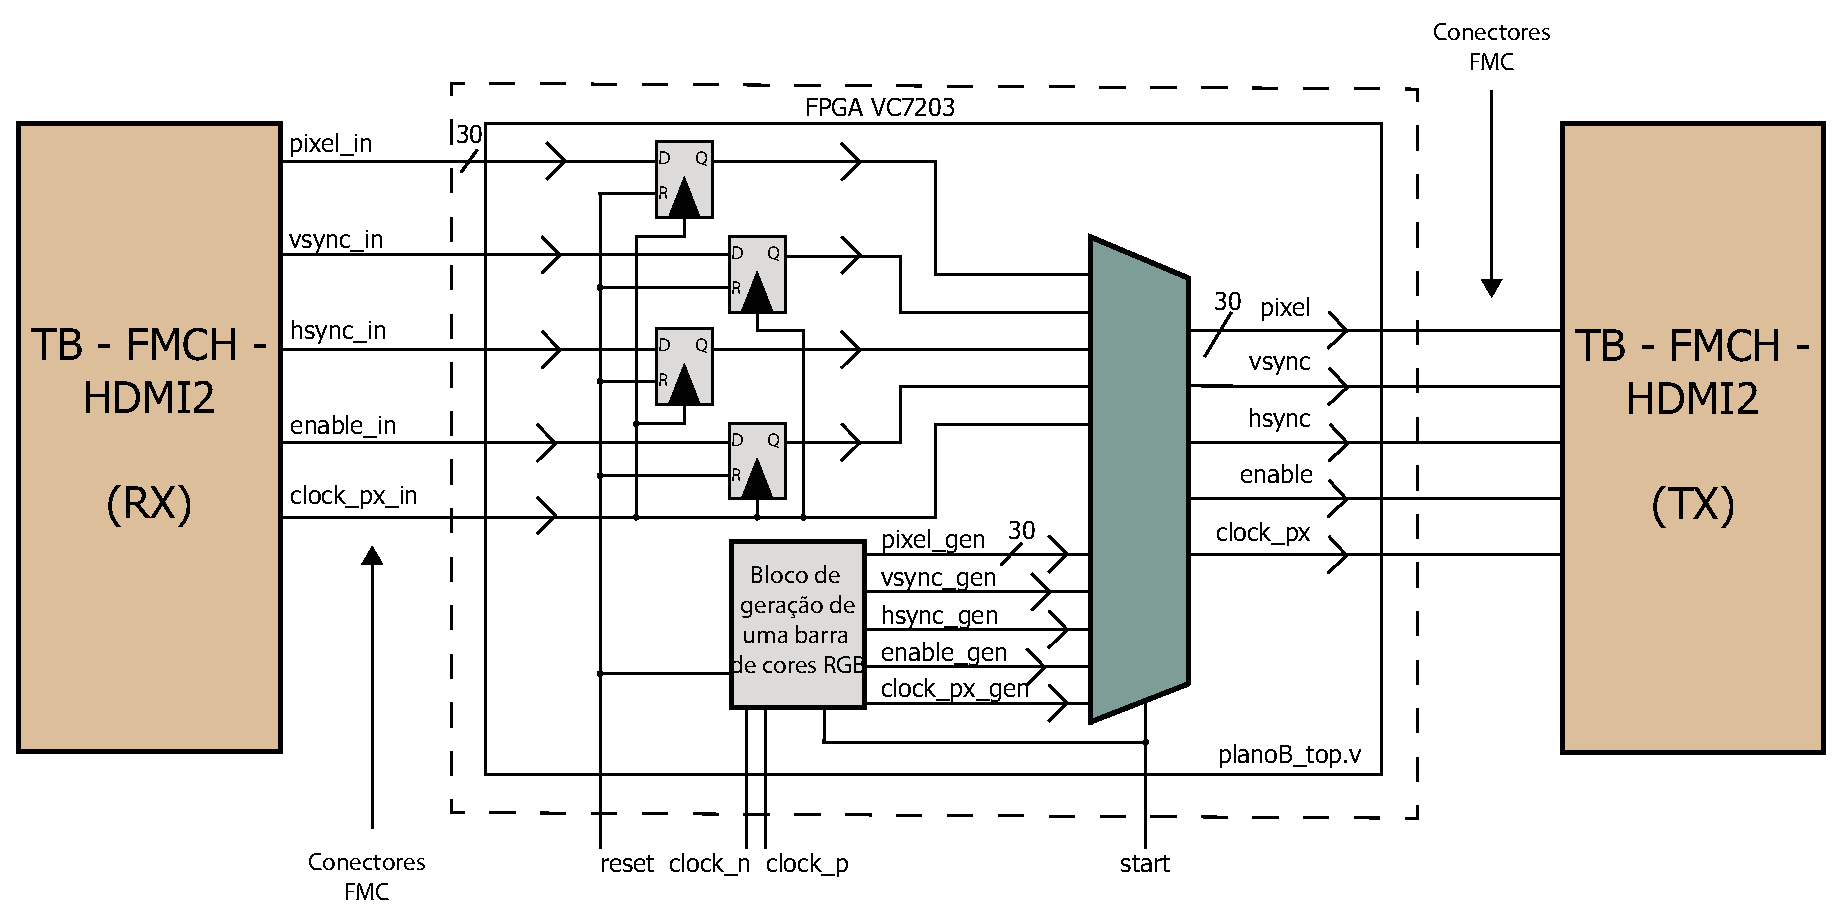
\includegraphics[width=1.0\textwidth]{planB1} 
			\caption{Diagrama de blocos da arquitetura}
			\label{fig:planoA}
		\end{center}
	\end{figure}

	\textbf{Disponível para o utilizador:}
	\begin{itemize}
		\item Botão \textbf{reset}: permite ao utilizador repor os dados originais do sistema;
		\item Interruptor \textbf{start}: permite ao utilizador definir o início da transmissão:
		\begin{itemize}
			\item \textbf{ON}: Transmissão ativa;
			\item \textbf{OFF}: Transmissão inativa;
		\end{itemize}
	\end{itemize}

	\section{Configuração do \textit{setup}}
	
	Na \cref{fig:setupA} está representado o \textit{setup} de teste que deve ser utilizado para esta arquitetura. A configuração de cada um dos componentes passa a ser de seguida descrito.
	
		\begin{figure}[h!]
		\begin{center}
			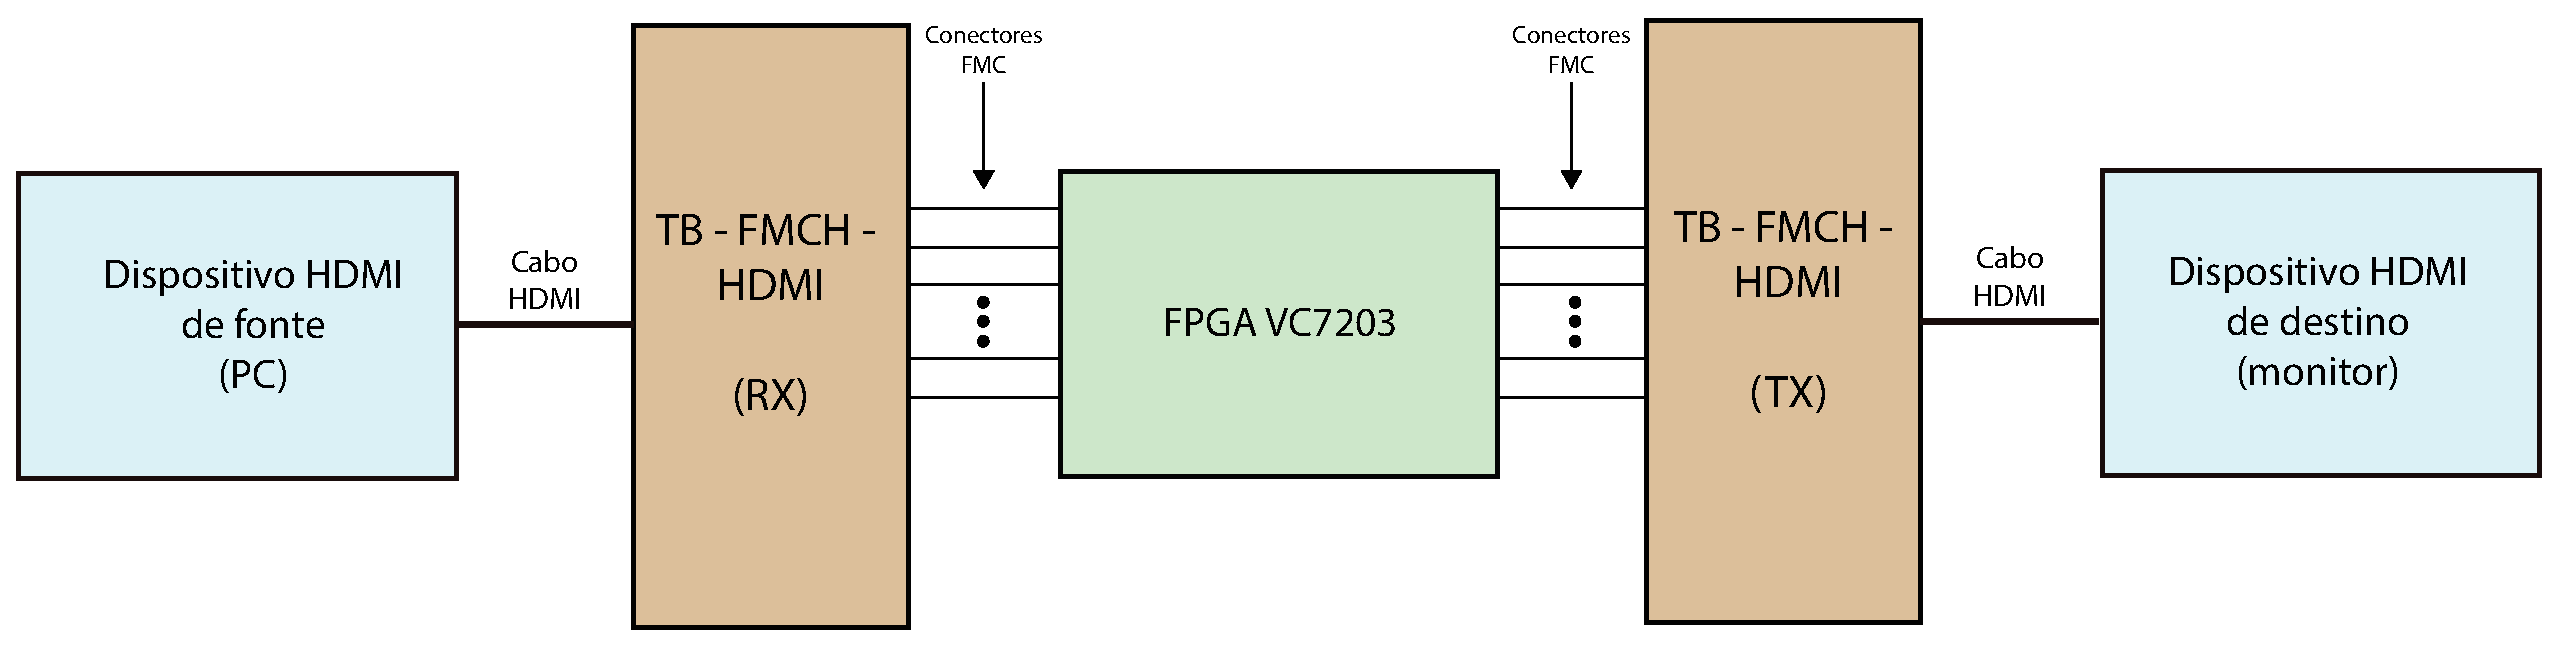
\includegraphics[width=0.8\textwidth]{planBsch} 
			\caption{\textit{Setup} de teste}
			\label{fig:setupA}
		\end{center}
	\end{figure}

	\subsection{TB-FMCH-HDMI TX}
	Estas placas devem estar configuradas por omissão. Para tal deve-se recorrer ao \textit{software iMPACT} e ainda ao programador JTAG (tal como indicado em \cite{R025}):
	\begin{itemize}
		\item O programador deve estar devidamente conectado à placa HDMI e ao computador;
		\item O \textit{software iMPACT} deve ser inicializado;
		\item Com o botão do lado direito do rato deve ser escolhida a opção ``Inicializar cadeia'';
		\item A PROM (\textit{Programmable read-only memory}) cujos detalhes podem ser encontrados em \cite{R026} da placa transmissora deve ser programada com o ficheiro com o nome ``\textit{tx\_fpga\_top.mcs}'' que se encontra na pasta ``\textit{finalFolder/HDMI\_programming/default}''.
	\end{itemize}
	
	
	\subsection{FPGA VC7203}
	
	A placa FPGA \textit{Virtex-7} deve ser programada com o \textit{bitstream} gerado pós-implementação da arquitetura no \textit{software} VIVADO.
	\begin{itemize}
		\item A FPGA deve estar devidamente conectada ao computador através da porta USB;
		\item Após inicializado, deve ser escolhida a opção ``\textit{Open Hardware Manager}'' no VIVADO;
		\item De seguida deve ser escolhida a opção ``\textit{Open New Target}'' dentro de ``\textit{Open Target}'';
		\item Na nova janela aberta deve-se seleccionar a FPGA \textbf{XC7VX485T-3} e terminar até a janela fechar;
		\item De seguida, selecciona-se com o botão do lado direito do rato o componente \textbf{XC7VX485T-3}, escolhendo-se a opção ``\textit{Program Device}'';
		\item Nessa janela é seleccionado o bitstream que tem o nome ``\textit{colorBarGenerator.bit}'' na pasta `\textit{finalFolder/planA}''
	\end{itemize}
	
	Mais informações sobre o \textit{software} VIVADO pode ser encontrado em \cite{R019}.


	\section{Utilização dos recursos da FPGA}
	
	Na Tabela \ref{table:recursosA} são apresentados os valores dos recursos utilizados pela FPGA nesta arquitetura (denominada por ``A'').
		\begin{table}[h!]
			\centering
			\caption{Recursos utilizados pela arquitetura na FPGA}
				\label{table:recursosA}
		%	\resizebox{\textwidth}{!}} \\ \hline
					\textbf{FF}                                            & 31                                      & 0,01                            \\
					\textbf{LUT}                                           & 59                                      & 0,02                            \\
					\textbf{I/O}                                           & 38                                      & 5,43         			   		\\
					\textbf{GT}                                            & 0                                       & 0                               \\ \hline
				\end{tabular}%
	%		}
		\end{table}
	
	Os valores percentuais ocupados pela mesma são muito baixos, possibilitando a expansão da mesma caso necessário. 
	
	%-------------------------------------------------------------------------
	%	BIBLIOGRAPHY
	%----------------------------------------------------------------------------------------
	
	\bibliographystyle{ieeetr}
	
	\bibliography{myrefs}
	
	
	%----------------------------------------------------------------------------------------
%	\begin{table}[h!]
%		\centering
%		\caption{Recursos utilizados pelas diferentes arquiteturas implementadas na FPGA}
%		\label{table:recursos_a_b_c}
%		\resizebox{\textwidth}{!}{%
%			\begin{tabular}{l|ll|ll|ll}
%				\hline
%				\multicolumn{1}{c|}{\multirow{2}{*}{\textbf{Recurso}}} & \multicolumn{2}{r|}{\textbf{Arquitetura A}}                                 & \multicolumn{2}{r|}{\textbf{Arquitetura B}}                                & \multicolumn{2}{r}{\textbf{Arquitetura C}}                               \\ \cline{2-7} 
%				\multicolumn{1}{c|}{}                                  & \multicolumn{1}{c}{\textbf{Utilização}} & \multicolumn{1}{c|}{\textbf{\%}} & \multicolumn{1}{c}{\textbf{Utilização}} & \multicolumn{1}{c|}{\textbf{\%}} & \multicolumn{1}{c}{\textbf{Utilização}} & \multicolumn{1}{c}{\textbf{\%}} \\ \hline
%				\textbf{FF}                                            & 31                                      & 0,01                             & 64                                      & 0,01                            & 59                                      & 0,01                            \\
%				\textbf{LUT}                                           & 59                                      & 0,02                             & 67                                      & 0,02                            & 27                                      & 0,01                            \\
%				\textbf{I/O}                                           & 38                                      & 5,43                             & 70                                      & 10                               & 103                                     & 14,71                           \\
%				\textbf{GT}                                            & 0                                       & 0                                & 0                                       & 0                                & 0                                       & 0                               \\ \hline
%			\end{tabular}%
%		}
%	\end{table}
%
%\begin{table}[h!]
%	\centering
%	\caption{Recursos utilizados pelas arquiteturas desenvolvidas de transmissão em série}
%	\label{table:recursos_planoD_planoE}
%	
%	\begin{tabular}{rllll}
%		\hline
%		\multicolumn{1}{c}{\multirow{2}{*}{\textbf{Recurso}}} & \multicolumn{2}{c}{\textbf{Arquitetura D}}                                 & \multicolumn{2}{c}{\textbf{Arquitetura E}}                               \\ \cline{2-5} 
%		\multicolumn{1}{c}{}                                  & \multicolumn{1}{c}{\textbf{Utilização}} & \multicolumn{1}{c|}{\textbf{\%}} & \multicolumn{1}{c}{\textbf{Utilização}} & \multicolumn{1}{c}{\textbf{\%}} \\ \hline
%		\multicolumn{1}{r|}{\textbf{FF}}                      & 566                                     & \multicolumn{1}{l|}{0,09}        & 710                                    & 0,12                            \\
%		\multicolumn{1}{r|}{\textbf{LUT}}                     & 486                                     & \multicolumn{1}{l|}{0,16}        & 590                                    & 0,19                            \\
%		\multicolumn{1}{r|}{\textbf{I/O}}                     & 44                                      & \multicolumn{1}{l|}{6,29}        & 78                                     & 11,14                           \\
%		\multicolumn{1}{r|}{\textbf{GT}}                      & 1                                       & \multicolumn{1}{l|}{2,86}        & 1                                      & 2,86                            \\ \hline
%	\end{tabular}%
%\end{table}

	
\end{document}